% $Id: synthetic.tex 1784 2016-01-06 14:56:56Z lv39 $
% $URL: https://forge.cornell.edu/svn/repos/lv39_papers/SynLBD/text/SJIAOS2015/synthetic.tex $

%\margincomment{LV}{Added this paragraph}
In this section, we describe a protection system which uses tabulations from synthetic data, in a variety of implementations, to compensate for the suppressions generated by the current protection system. They should be considered extensions or complements to the current protection methods, since we describe and implement them within the constraints of the current system. In particular, our definition of sensitive cells is driven entirely by the current protection system. For comparison purposes, we also (partially) implement an  alternate protection system, multiplicative noise infusion. 

\subsection{Synthetic Data Tabulations}


The \ac{SynLBD} \cite{SynLBD20} is a synthetic dataset on establishments with proven analytic 
validity along several critical dimensions \cite{KinneyEtAl2011}. Additional improvements are 
currently being developed \cite{KinneyEtAl2013,CES-WP-2014-12}. A growing number of 
researchers have used the \ac{SynLBD}, and their continued use contributes to the 
improvement of the \ac{SynLBD}. 

The use of the \ac{SynLBD} for the purposes outlined in this paper is particularly appealing, 
because its analytic validity has been independently established, while maintaining a high level 
of data privacy. Based on the variables already available on the released \ac{SynLBD}, tabulations that 
use the \ac{SynLBD} as an input presumably require no additional disclosure avoidance review. %\margincomment{re MHS}{This was already addressed.}
Only tabulations involving state and sub-state geography should require 
additional review since geographic variables were removed from the disclosure request that 
approved the  release to the public of the SynLBD.%
\footnote{The Census Disclosure Review Board has not pronounced itself on the disclosure 
avoidance methodology proposed here as of December 2015.}
 
The available \ac{SynLBD} is released as a single implicate, and by design, may distort an analysis by a potentially large an amount. The use of additional implicates for the purposes of BDS table creation may be desirable and will be assessed in later work. 

%\margincomment{Lars}{Needs to be rewritten}
In this paper, we propose and evaluate several algorithms that complement the existing 
\ac{BDS} disclosure avoidance methodology (primary and secondary suppression, PSS). In all 
cases, we allow the PSS methodology to determine which cells are sensitive. Once identified, 
sensitive cells as well as some additional cells are modified using tabulations based on synthetic 
establishments.  

The first algorithm, which we will call the ``drop-in algorithm'', simply replaces a cell that has 
been suppressed with its synthetic-data equivalent, i.e., the equivalent table cell from a 
tabulation based on the \ac{SynLBD} alone. The second algorithm, called 
``forward-longitudinal algorithm'', is slightly more complicated. At any point in time $t$, if a 
(expanded) suppression algorithm identifies a cell that \emph{would} be suppressed under 
PSS, all 
establishments that contribute to that cell in  time period $t$ are replaced by synthetic 
establishments that match on certain characteristics $Z$ in periods $t-p$ through $t$, for $t$ 
and the next $n$ periods. Synthetic and observed values are then tabulated to create the 
release statistics. To smooth the phasing out of the synthetic establishments, we define weights 
$w(n)$ that decline monotonically from unity to zero for synthetic establishments, and increase 
correspondingly for real establishments. 
If $Z$ 
describes only the margin characteristics for the table in question 
(denoted by $k$ below), and not any additional characteristics, and for $p=n=0$, the algorithm 
is similar to the ``drop-in'' algorithm, but creates consistent higher-level tables automatically. 
On the other hand, the ``forward-longitudinal algorithm'' cannot be done post-publication 
without the re-release of historical tabulations.

In this paper, we will restrict ourselves to $p=0$ and $n=\lbrace 0,4 \rbrace$ in order to assess the 
time-consistency of the proposed algorithms for a single implicate.
%\margincomment{Re MHS}{This had already been addressed.}
We have 
previously assessed the impact of Algorithm 1 (defined below)  \cite{psd2014a}.
Assessing the impact of using multiple implicates as well as identifying 
acceptable values of $Z$, $p$, and $n$ is deferred to  future work.

\subsection{Definitions}
The variable of interest is establishment employment $e_{jt}$, with establishments indexed by 
$j$ and years indexed by $t$. All other variables (job creation and destruction from 
establishment entry, exit, expansion and contraction) are derived from that basis. For instance, 
an establishment is ``born'' at time $t$ if employment is positive for the first time in $t$:
\begin{eqnarray}
\label{eq:e_birth}
birth_{jt} &=& \left \lbrace 
\begin{array}{rl}
1 &\mbox{if}~~  e_{jt} > 0 ~~ \mbox{and}  ~~e_{jt-s} = 0 ~~\forall s\geq 1~~\\
0 &\mbox{otherwise}
\end{array} \right .
\end{eqnarray}
We will denote aggregations using capital letters, so (national) employment is denoted as
%\margincomment{Re MHS}{Corrected confusing switch in notation.}
\begin{equation}
\label{eq:national_e}
E_{\cdot t} = \sum_{j=1}^J e_{jt}
\end{equation}
and (national) births are
\begin{equation}
\label{eq:national_birth}
Birth_{\cdot t} = \sum_{j=1}^J birth_{jt}.
\end{equation}
An establishment $j$ has a vector of  time-invariant and time-varying
characteristics $k_t(j)$, such as industry and geographic location (time-invariant), but also 
derived 
characteristics, such as establishment or firm age and size. In a slight abuse of notation, $j \in 
K_t^\prime$ describes the set of firms at time $t$ such that $k_t(j)=k^\prime$.   Generically, 
\begin{equation}
\label{eq:sum_X}
X_{k^\prime t} =  \sum_{j \in K_t^\prime} x_{jt}
\end{equation}
describes the different aggregations across establishments having characteristics $k^\prime$ at 
time $t$, for instance aggregations by establishment age or metropolitan areas, referred to as 
``confidential BDS'' (\textbf{BDS$^{conf}$}).
%

For any establishment $j$, the synthesized version of variable $x_{jt}$ (from a single implicate) is 
denoted $\tilde{x}_jt$. The vector $\tilde{k}_t(j)$ describes the set of characteristics when using 
the synthetic dataset, which will generally differ from $k_t(j)$ because time-varying derived 
characteristics such as age and size will differ (at this time, neither industry nor geography are 
synthesized). We designate the set of  establishments $j$ with synthetic characteristics 
$\tilde{k}_t(j)$ as $\tilde{K}_t^\prime$, and will refer to them as  ``synthetic 
establishments.''  Aggregations across synthetic establishments are
\begin{equation}
\label{eq:sum_X_synth}
\tilde{X}_{k^\prime t} =  \sum_{j \in \tilde{K}_t^\prime} \tilde{x}_{jt}
\end{equation}
and will be referred to as ``synthetic BDS'' (\textbf{BDS$^{(s)}$}).

Finally, suppression rules for (aggregate) variable $X$ are captured by $I_{t}^X$, such that the 
releasable variable $X^o$  under the current regime (PSS) can be described by

%\begin{equation}
%\label{eq:supp_x}
%X_{k^\prime t}^o = X_{k^\prime t}  I_{t}^X 
%\end{equation}
\begin{eqnarray}
\label{eq:supp_x}
X_{k^\prime t}^o &=& \left \lbrace 
\begin{array}{rl}
X_{k^\prime t} &\mbox{if}~~  I_{kt}^X = 1 \\
\mbox{missing} &\mbox{otherwise}
\end{array} \right .
\end{eqnarray}

For later 
reference, we denote the tabulations created as per (\ref{eq:supp_x}) as \textbf{BDS$^{(0)}$}.
%We will denote by $K_t^\prime \subset K$ the subset of the domain of $K$, such as certain industries, or age categories within certain geographic areas, so that $J_t^j \in K_t^\prime$ 

\subsection{Algorithm 1: Drop-in}

We can now express the ``drop-in'' algorithm, leading to the released variable $X^{(i)}$, as:
\begin{algorithm}
%\caption{(n=0) Drop-in}
\label{alg1n}
\begin{algorithmic}
\If {$I_{t}^X = 0$ }
        \State {$X_{k^\prime t}^{(i)} =\tilde{X}_{k^\prime t} $}
\Else
    \State {$X_{k^\prime t}^{(i)} = X_{k^\prime t} $}
\EndIf
\end{algorithmic}
\end{algorithm}

Thus, simply computing a ``SynBDS'', based on the \ac{SynLBD}, in parallel to the computation 
of the \ac{BDS}, based on the confidential \ac{LBD}, and replacing suppressed cells with their 
fully synthetic counterparts, yields a dataset without missing cells. Note that we have assumed 
the existence of only one synthetic implicate; the use of multiple synthetic implicates would 
replace the second component of Algorithm~1 with  
$X_{k^\prime t}^{(i)} = \frac{1}{\ell} \sum_{l=1}^{\ell} \tilde{X}_{k^\prime t l} $, the average across 
$\ell$ 
implicates. In 
general, increasing the number of implicates will improve the analytic validity, but reduce the 
protection provided by the synthesis process. 

Because no time-consistency is imposed, this method can lead to seam biases or higher 
intertemporal variance. Furthermore, only interior cells are adjusted, but no margins are 
corrected, likely leading to discrepancies in the global table structure. Raking would solve that 
issue, but is not explored here. %We will return to this issue in Section~\ref{sec:analysis}. 

%\margincomment{LV}{Additional paragraph for the smoothed drop-in}
In order to smooth the time-series generated by this process, and to provide a comparison to 
the microdata-based smoothing outlined later in this section, we generalize the above algorithm 
to combine not just synthetic tabulations in periods with suppression, but also in later periods. 
Thus, in periods that follow a period with $I_{t}^X = 1$, we average synthetic tabulations with 
non-suppressed tabulations, for up to $n$ periods:
%\addtocounter{algorithm}{-1}
%\newpage
\begin{algorithm}
%\caption{Weighted Drop-in}
{\bf Algorithm 1: Weighted Drop-in}
\hrule
\label{alg1}
\begin{algorithmic}
\State {$s^* = min_{s \in [0,n]} $ s.t. $I_{t-s}^X = 0$ }
\If { $n>0$ and $\exists s^*$ }
    \State {$X_{k^\prime t}^{(i)} =  \frac{s^*}{n} X_{k^\prime t}  
               + \left (1-\frac{s^*}{n} \right ) \tilde{X}_{k^\prime t} $}
\ElsIf { $n=0$ and $I_{t}^X = 0$}
    \State {$X_{k^\prime t}^{(i)} =  \tilde{X}_{k^\prime t} $}
\Else
        \State {$X_{k^\prime t}^{(i)} ={X}_{k^\prime t} $}               
\EndIf
\end{algorithmic}
\end{algorithm}

For $n=0$ this reduces to the prior expression. 
For later 
reference, we denote the tabulations created by Algorithm~1 as \textbf{BDS$^{(i)}$} 
in its general form, and as \textbf{BDS$^{(in)}$}  when $n=0$.
%\margincomment{Re MHS}{I hesitated, because when using $^{2}$ it might be confused for "squared", whereas $^{ii}$ is not ambiguous}

\subsection{Algorithm 2: Forward-longitudinal}

In part to address the possible time-inconsistencies we propose an 
alternative algorithm.  In order to minimize future seam issues, we downweight or remove 
establishments (or 
firms) that 
contribute to sensitive cells of tabulations with characteristics $k^\prime t$, for $t$ and the next 
$n-1$ periods. These establishments are (partially) replaced by  synthetic establishments that 
match on 
characteristics $k^\prime t$, and we simply replace the observed values in the database $x_{js}$ 
with the synthetic values $\tilde{x}_{js}$ (for all variables), for $s=t,\dots,t+n$.  %
%
For convenience, 
denote by $J_{k^\prime t}^-$ the set of establishments that are to be excluded from tabulations at time $t$, and $J_{k^\prime t}^+$ the set of synthetic establishments that are added to the 
tabulations as replacements. We construct $J_{k^\prime t}^-$ by first adding establishment identifiers that meet the suppression conditions $I^X_{kt}$ at time $t$. In addition, we assign establishments to 
$J_{k^\prime s}^-$ for the $n$ periods after a cell stops being sensitive as well. Formally, we  add 
those same establishments to ``future''  $I^X_{ks}$, for $s \in [t+1,t+n]$ if $n>0$. Thus, at any 
point in time $t$, the set $J_{k^\prime t}^-$ contains establishments that met suppression 
conditions now and in the past, i.e.,   in $[t-n,t]$.   
%\margincomment{Re MHS}{Moved the sentence here, clarified (hopefully) language.}
%
In order to ``smooth'' the tabulated data, we specify  a 
per-establishment weight $w_{js} \in [0,1]$, applied to the observed data, that increases from 
$0$ in $t$ to $1$ in $t+n$, 
and  a per-establishment weight $\tilde{w}_{js}$, applied to the synthetic data, that decreases 
from $1$ in $t$ to $0$ in 
$t+n$, thus ``blending in''  the real establishments, and ``blending out'' the synthetic 
establishments. Setting $w_{js} = 0, s \in [t,t+n-1]$ and $\tilde{w}_{js}=1, s \in [t,t+n-1]$ effectively 
removes the real establishments from the tabulation, being completely  replaced by the synthetic 
establishments.
%
In its simplest 
form, the algorithm can be expressed as

%\addtocounter{algorithm}{1}
\begin{algorithm}
%\caption{Forward-longitudinal}
{\bf Algorithm 2: Forward-longitudinal}
\hrule
\label{algorithm:2}
\begin{algorithmic}
\State {Compute: $X_{k^\prime t} = \sum_{j \in K_t^\prime} x_{jt}$}
\State{Compute: $I_{t}^X$}
\If {$I_{t}^X = 0$  }
   \State {// Suppression condition met for cell $k^\prime$}
    \State {Assign all $j \in K_t^\prime$ to $J_{k^\prime s}^-$ for $t \leq s \leq t+n$}
    \State {Assign all $j \in \tilde{K}_t^\prime$ to $J_{k^\prime t}^+$ for $t \leq s \leq t+n$}
\EndIf
\State { Compute: %
$$
X_{k^\prime t}^{(iiw)} = 
               \sum_{j \in \left \lbrace K_t^\prime \cap J_{k^\prime t}^+ \right \rbrace }
                               \tilde{w}_{jt} \tilde{x}_{jt} 
	          +
	          \sum_{j \in  K_t^\prime \wedge j \in J_{k^\prime t}^-  }
	                                  w_{jt}  {x}_{jt} 
	          +
	          \sum_{j \in  K_t^\prime \wedge j \notin J_{k^\prime t}^-  }
	                                         {x}_{jt} 
$$}

\end{algorithmic}
\end{algorithm}
%
where the first component is the (possibly down-weighted) sum of synthetic data, the second 
component is the (up-weighted) sum of observed establishments in periods after they are no 
longer part of sensitive cells, and the third component is sum of establishments that were not 
part of sensitive establishments in the past (or outside of the window $[t-n,t]$). 

For $n=\infty$, $J_{t}^-$ is an absorbing set, which seems undesirable. For $n=0$, this is similar 
to, 
but not equal to Algorithm~1. Note that in contrast to Algorithm~1, all higher level tabulations 
are consistent, since the replacement occurs at the microdata level, not at the tabulation cell 
level.

Consider the case for period $s$ for which $I_{s}^X=1$ and $I_{s-1}^X=0$, i.e., the suppression 
conditions no longer apply. By assignment in period $s-1$, some LBD establishments are still 
assigned to $J_{k^\prime s}^-$, and some synthetic establishments are still part of $ J_{k^\prime 
t}^+$. However, new LBD establishments that are identified by $k^\prime$ are counted in 
$X_{k^\prime t}^{(ii)}$ by virtue of the second sum. Equivalently, establishments (synthetic or 
real) that move out of $k^\prime$ (because they age or grow out of the category) naturally drop 
out of $X_{k^\prime t}^{(ii)}$. Note that because we condition on $J_{k^\prime}$, synthetic 
establishments that naturally exit tabulation cell $k^\prime$ are not counted toward an 
alternative tabulation cell $k^\star$, unless that cell is \textit{also} a candidate for suppression. 
For reference, we denote the tabulations created by Algorithm~2 as \textbf{BDS$^{(ii)}$}.


\subsection{Multiplicative Noise Infusion}
%\margincomment{LV}{This entire section added}
Multiplicative noise infusion was originally proposed by \cite{EvansZayatzSlanta1998}. Implementations include the \ac{QWI} \cite{AbowdEtAl2009} and the \ac{CBP}. We apply multiplicative noise to employment counts and payroll measures (although our analysis in this paper only focuses on employment-based measures). 

Multiplicative noise is drawn  for each establishment $j$ 
from a bilateral ramp distribution:%
\begin{equation}\arraycolsep=1.4pt\def\arraystretch{2.2}
	p\left( {\delta _{j}}\right) =\left\{ {{%
			\begin{array}{ccl} 
			\dfrac{ {1+ b - \delta } }{\left( {b - a} \right)^2}
					&,&\;\delta \in \mbox{ }\left[ {1+a,1+b} \right] \\ 
				\dfrac{ {\delta - (1 - b)} }{\left( {b - a} \right)^2} 
				&,&\;\delta \in \left[ {1 - b,1 - a} \right] \\ 
				0&,&\;\mbox{ otherwise } \\
				 \end{array}%
		}}\right. 
	\end{equation}%
%	\begin{equation}
%		F\left( {\delta _{j}}\right) =\left\{ {{%
%				\begin{array}{*{20}c} {\mbox{0},\;\delta < {2-b} } \\ {{\left[ {\left( {\delta + b - 2} \right)^2} \right]} \mathord{\left/ {\vphantom {{\left[ {\left( {\delta + b - 2} \right)^2} \right]} {\left[ {2\left( {b - a} \right)^2} \right]}}} \right. \kern-\nulldelimiterspace} {\left[ {2\left( {b - a} \right)^2} \right]},\;\delta \in \left[ {2 - b,2 - a} \right]\mbox{ }} \\ {\mbox{0.5}, \;\delta \in \mbox{ }\left( {2-a,a} \right)\mbox{ }} \\ {\mbox{0.5} + {\left[ {\left( {b - a} \right)^2 - \left( {b - \delta } \right)^2} \right]} \mathord{\left/ {\vphantom {{\left[ {\left( {b - a} \right)^2 - \left( {b - \delta } \right)^2} \right]} {\left[ {2\left( {b - a} \right)^2} \right]}}} \right. \kern-\nulldelimiterspace} {\left[ {2\left( {b - a} \right)^2} \right]},\;\delta \in \mbox{ }\left[ {a,b} \right]\mbox{ 
%						}} \\ {\mbox{1}, \;\delta > {b} } \\ \end{array}}}\right. 
%		\end{equation}%
		
\noindent where $a={c}/{100}$ and $b={d}/{100}$ are constants chosen
		such that the true value is distorted by a minimum of $c$ percent and a
		maximum of $d$ percent. This produces a random noise factor centered around 1 with
		distortion of at least $c$ and at most $d$ percent. Figure~\ref%
		{fig:fuzzgraph} depicts such a distribution.  The noise factor is drawn only once,  and 		retained for all time periods after the initial assignment. For this exercise, we set $c=10$ and $d=25$ percent as plausible numbers, for illustration only. Note that these numbers are in general confidential, and we have no knowledge of the actual parameters used in \ac{QWI} and \ac{CBP}. Both \ac{QWI} and  \ac{CBP} use  slightly more complex noise infusion algorithms that takes into account the firm structure and table structure, and include suppression for the smallest cells where multiplicative noise provides insufficient protection. None of those additional features are implemented here.
%
We denote the tabulations protected by noise infusion as \textbf{BDS$^{(n)}$}.
		
		
%\begin{figure}
%	\centering
%	\caption{Empirical distribution of noise\label{fig:fuzzgraph}}
%	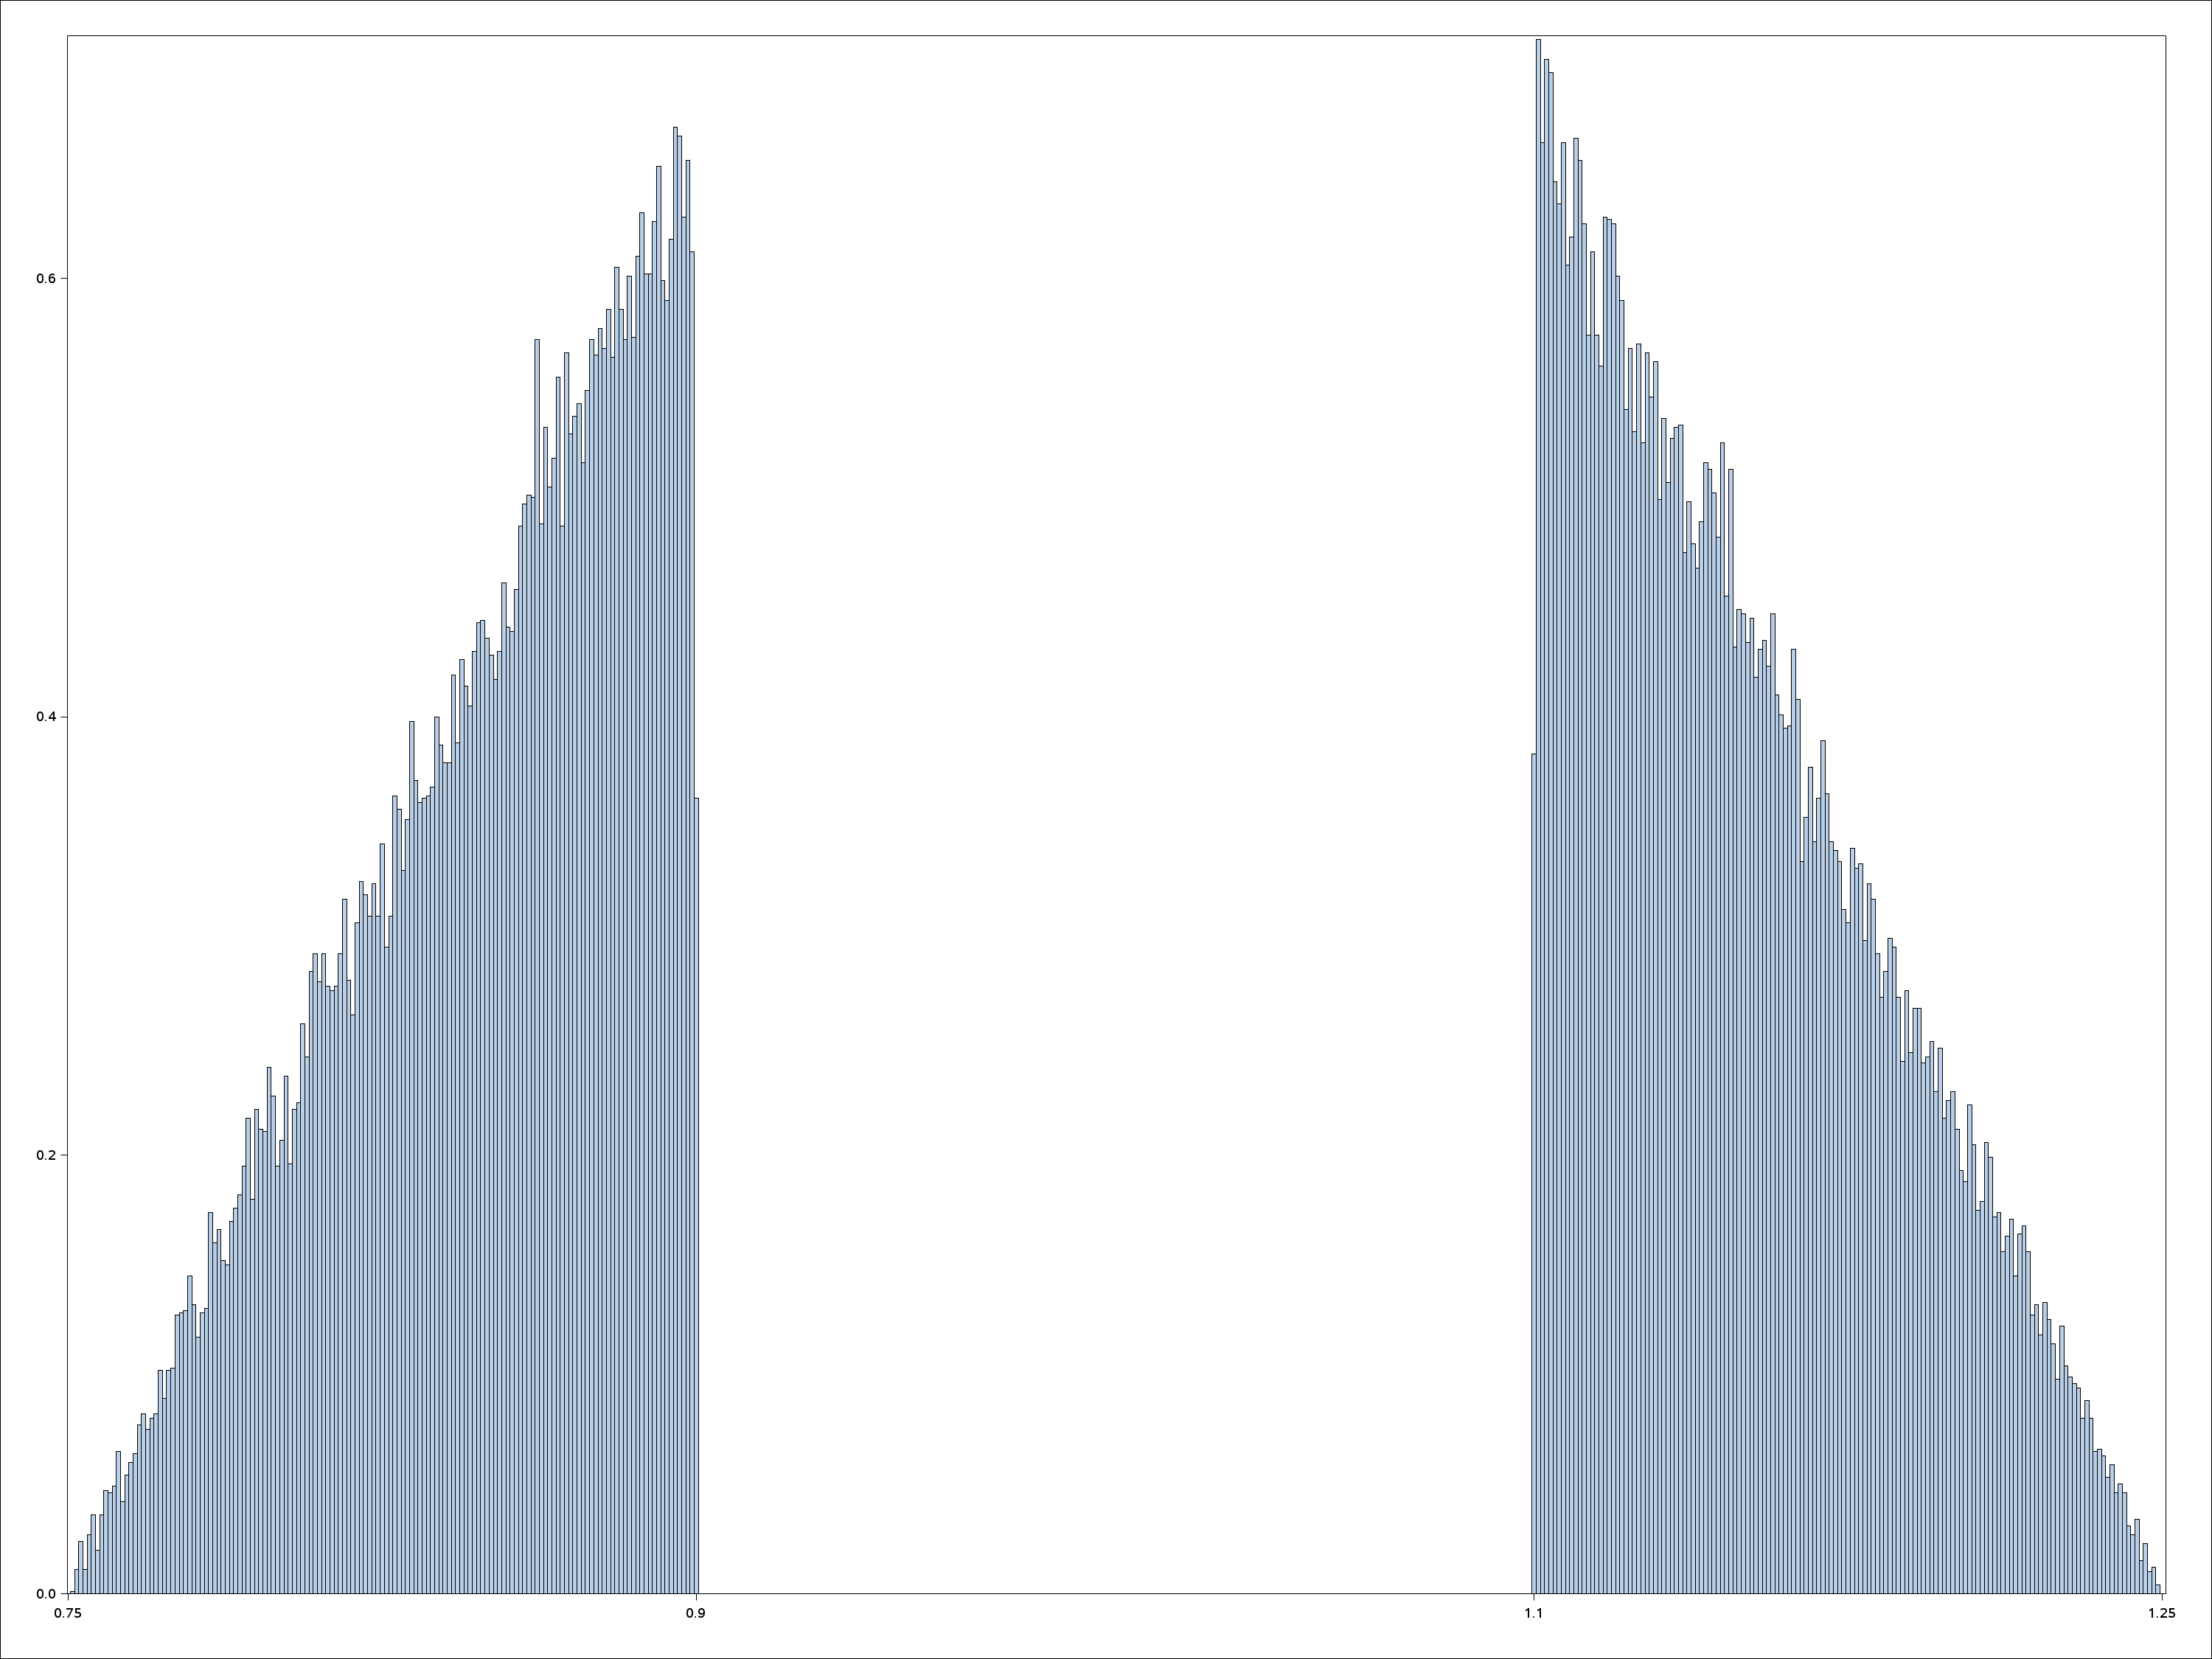
\includegraphics[width=0.5\textwidth]{SGPlot.png}
%\end{figure}

